\section{Semantik}

Die semantische Auswertung der abstrakten Syntax wird im
PrincipleWriter vom Evaluatormodul \"ubernommen. Auch wenn im
Programmablauf des PrincipleWriters der Optimizer vor dem Evaluator
kommt, werden wir uns zuerst den Evaluator anschauen, da die
Funktionalit\"at des Optimizer so einfacher zu verstehen ist.

Die Aufgabe des Evaluators ist es, aus der abstrakten Syntax mit Hilfe
von semantischen \"Uberf\"uhrungsregeln den Mozart/Oz-Code der
Prinzipien zu generieren. Der generierte Mozart-Code greift auf
Funktionen aus dem Modul {\tt PW.oz} zur\"uck, um die logischen
Operationen (Quantoren, Konnektive etc.) zu implementieren.  Der
Evaluator \"ubergibt den Record, der die abstrakte Syntax enth\"alt,
an die Evaluierungsfunktion, die eine Liste von Tupeln der Form
\begin{center}
{\tt Name\#DV\#Constraints}
\end{center}
zur\"uckgibt. Hierbei ist {\tt Name} der Prinzipienname, {\tt DV}
sind die Dimensionsvariablen, \"uber die das Prinzip abstrahiert, und
{\tt Constraints} der Mozart/Oz-Code f\"ur die logische Formel.  Aus
jedem dieser Tupel wird dann eine Prinzipiendefinition und ein
Node-Constraint-Funktor generiert und als zwei Dateien gespeichert,
die direkt in die XDK-Prinzipienbibliothek eingegliedert werden
k\"onnen.

\subsection{Semantik der PWUL}

Die Semantik der PrincipleWriter User Language wird durch eine
Interpretationsfunktion definiert, die aus den Regeln aus
Anhang~\ref{semantik} besteht, die die Formel rekusiv auswertet
innerhalb der Umgebung $(V,M,T)$. Hierbei ist:
\begin{itemize}
\item $V$ ein Record mit drei Feldern:
$$V= \left \{ \begin{array}{r c l}
a & : & \left \{ \begin{array}{c}\text{VarName:Oz-Atom-Name}\\ \vdots \end{array} \right \} \\
i & : & \left \{ \begin{array}{c}\text{VarName:Oz-Integer-Name}\\ \vdots \end{array} \right \} \\
n & : & \left \{ \begin{array}{c}\text{VarName:Oz-Node-Name}\\ \vdots \end{array} \right \} \\
\end{array}
\right \}$$ eines f\"ur atomare Variablen, eines f\"ur numerische
Variablen und eines f\"ur Knotenvariablen. Jedes Feld enth\"alt einen
Record aus Paaren, deren erster Wert der Variablenname ist und der
zweite die Entsprechung in den zu generierenden Mozart/Oz-Constraints.
\item $M$ ein Modus. Bei der Interpretation muss eine Variable je nach
Umgebung atomar, numerisch oder als Knoten interpretiert werden. Der
Modus $M={a,i,n}$ bestimmt, wie die Variable interpetiert wird.
\item $T$ eine Typannahme.
\end{itemize}

Die Funktionsweise der Regeln wollen wir anhand einiger Beispiele
erkl\"aren.

\subsubsection{Quantoren}

Die Interpretation von Quantoren wollen wir am Beispiel des
$\exists$-Quantors erkl\"aren. Die Interpretationsregel sieht so aus:

\begin{flushleft}
\begin{tabular}{l}
\inter{exists ~ Constant::Dom:Form} = \\
\begin{tabular}{@{\hspace{40pt}}l}
if Dom == node then\\
\tab NodeRecV = Constant\#{\tt 'NodeRec'}\\
in\\
\tab {\tt '\{PW.existsNodes NodeRecs}\\
\ttab {\tt fun \{\$ '\#}NodeRecV{\tt \#'\}'\#}\\
\ttab \tab \fullinter{\left( \begin{array}{c}V.n \cup \{Constant:NodeRecV\}\end{array}\right)}{M}{T}{Form}{\tt \#}\\
\ttab {\tt end\}'}\\
else\\
\tab AV = Constant\#{\tt 'A'}\\
\tab IV = Constant\#{\tt 'I'}\\
in\\
\tab {\tt '\{PW.existsDom \{T2Lat '\#}Dom{\tt \#'\}}\\
\ttab {\tt fun \{\$ '\#}AV{\tt \#}IV{\tt \#'\}'\#}\\
\ttab \ttab \ttab \fullinter{\left( \begin{array}{c}V.a \cup \{Constant:AV\}\\
V.i \cup \{Constant:IV\}\end{array}\right)}{M}{T}{Form}{\tt \#}\\
\ttab {\tt end\}'}\\
end\\
\end{tabular}
\end{tabular}
\end{flushleft}

Es wird unterschieden, ob \"uber einen Knoten oder eine andere
Dom\"ane quantifiziert wird. Da die Knotenmenge in jedem Node
Constraint Funktor {\tt NodeRecs} hei{\ss}t, kann der Mozart/Oz Code
direkt generiert werden. Die Funktionsbibliothek {\tt PW} stellt einen
$\exists$-Quantor \"uber die Knoten zur Verf\"ugung, der die
Knotenmenge als Argument hat (immer {\tt NodeRecs} in
Node-Constraint-Funktoren), und die Funktion, die f\"ur einen Knoten
wahr sein muss. Der Rumpf dieser Funktion ergibt sich aus der
Interpretation der Formel {\tt Form} innerhalb der bisherigen
Umgebung, der die Variable {\tt Constant} und ihre Entsprechung im
generierten Mozart-Code (Constant\#{\tt 'NodeRec'}) hinzugef\"ugt
wird.

Wird \"uber eine andere Dom\"ane als \"uber Knoten quantifiziert, muss
zuerst ein Name f\"ur die Dom\"ane generiert werden. Der
$\exists$-Quantor \"uber nicht-Knoten-Mengen, der von der
PW-Bibliothek bereitgestellt wird, bekommt den generierten Namen und
eine Funktion als Argumente. Die Variable {\tt Constant} hat in diesem
Fall zwei Entsprechungen im generierten Mozart-Code: Constant\#{\tt
  'A'} (quantifiziertes Element als Oz-Atom) und Constant\#{\tt 'I'}
(als Oz-Integer). Beide werden u.U.\ von der {\tt
  PW}-Funktionsbibliothek gebraucht.

\subsubsection{Konstanten und Variablen}

\begin{figure}
\begin{flushleft}
\begin{tabular}{l}
\inter{Constant} =\\
\begin{tabular}{@{\hspace{40pt}}l}
if \{Char.isAlpha \{Atom.toString\ Constant\}.1\} andthen\\
\tab \{Char.isUpper \{Atom.toString\ Constant\}.1\} andthen\\
\tab \{List.all \{Atom.toString Constant\}\\
\ttab fun \{\$ Ch\} \{Char.isAlpha Ch\} orelse \{Char.isDigit Ch\} end\}\} then\\
\tab if M == i then\\
\ttab if T == node then\\
\tab\ttab V.n.Constant.index\\
\ttab else\\
\tab\ttab V.i.Constant\\
\ttab end \\
\tab elseif M == a then \\
\ttab V.a.Constant\\
\tab else\\
\ttab V.n.Constant\\ 
\tab end\\
else \\
\tab if M == i then\\
\ttab {\tt '\{\{T2Lat '\#}T{\tt \#'\}.a2I '\#}Constant{\tt \#'\}'}\\
\tab elseif M == a then\\ 
\ttab Constant\\
\tab end\\
end\\
\end{tabular}
\end{tabular}
\end{flushleft}
\caption{Interpretation von Konstanten und Variablen}
\label{consem}
\end{figure}

Bei der Interpretation von Konstanten und Variablen muss erst
festgestellt werden, ob {\tt Constant} eine Konstante oder eine
Variable ist, da der kontextfreie Parser das nicht unterscheidet.
Variablen beginnen immer mit einem Gro{\ss}buchstaben und d\"urfen nur
Buchstaben und Zahlen enthalten. Alles andere sind Konstanten.

Bei der Interpretation einer Variablen wird anhand der Umgebung
festgestellt, ob es sich um eine atomare, eine numerische oder eine
Knotenvariable handelt. Die Interpretation gibt dann die
Mozart/Oz-Entsprechung des Variablennamens aus dem Record $V$
zur\"uck.

\subsubsection{Logische Operatoren und Mengenoperatoren}

\begin{figure}

\begin{center}
\begin{tabular}{l}
\inter{Expr_1 ~ union ~ Expr_2 ~ = ~ Expr_3} =\\
\begin{tabular}{@{\hspace{40pt}}l}
{\tt '\{PW.union '\#}\\
\tab \fullinter{V}{i}{T}{Expr_1}{\tt \#' '\#}\fullinter{V}{i}{T}{Expr_2}{\tt \#' '\#}\fullinter{V}{i}{T}{Expr_3}{\tt \#\}'}
\end{tabular}
\end{tabular}
\end{center}
\caption{Interpretation f\"ur die Vereinigung von Mengen}
\label{semunion}
\end{figure} 

Bei logischen Operatoren und Mengenoperatoren werden zuerst die
Unterb\"aume interpretiert, und diese Interpretationen dann als
Argumente f\"ur Funktionsapplikationen aus der {\tt PW}-Bibliothek
eingef\"ugt. Die {\tt PW}-Bibliothek stellt f\"ur jeden logischen Operator
und jede Mengenoperation eine Funktion zur Verf\"ugung. Da Mengen in
XDK immer Mengen von nat\"urlichen Zahlen sind, muss die Auswertung
der Unterb\"aume eines Mengenoperators im Modus $M=i$ interpretiert
werden. Abbildung~\ref{semunion} zeigt die Regel f\"ur die Vereinigung
von Mengen.

\subsection{Beispiel: Disjunktheit von Unterb\"aumen mit
  unterschiedlichem Label}
\begin{figure}
\begin{center}
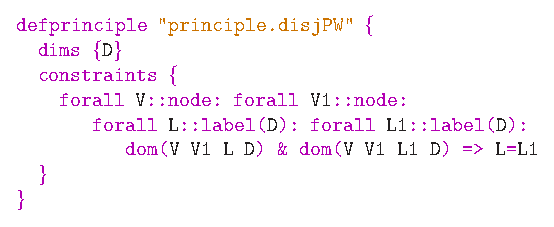
\includegraphics[scale=1.0]{eps/disj}
\end{center}
%% \begin{verbatim}
%% defprinciple "principle.disjPW" {
%%   dims {D}
%%   constraints {
%%     forall V::node: forall V1::node:
%%        forall L::label(D): forall L1::label(D):
%%           dom(V V1 L D) & dom(V V1 L1 D) => L=L1
%%   }
%% }
%% \end{verbatim}
\caption{Prinzip Disjunktheit von Teilb\"aumen mit unterschiedlichem
  Label in PWUL}
\label{disjunktPW}
\end{figure}
Als Beispiel wollen wir uns die Evaluierung eines Teils des
Baumprinzips anschauen. In Abbildung~\ref{disjunktPW} ist der
Constraint zu sehen, der fordert, dass zwei Unterb\"aume eines Knotens
mit gleichem Label disjunkt sein m\"ussen.

Die Interpretationsfunktion extrahiert zuerst den Namen des Prinzips.
Danach baut sie einen Record, der Dimensionsvariablen auf konkrete
Dimensionen abbildet, auf die zur Laufzeit mit der Funktion {\tt
  Principle.dVA2DIDA} zugegriffen werden kann. Im generierten
Mozart/Oz-Code wird im Beispiel die Dimensionsvariable {\tt D} immer
durch {\tt \{Principle.dVA2DIDA \verb=\='D\verb=\='\}}
repr\"asentiert.

Die beiden ersten Quantoren, die \"uber Knoten quantifizieren, werten
wie vorher beschrieben aus:
\begin{verbatim}
{PW.forallNodes NodeRecs
 fun {$ VNodeRec}
    {PW.forallNodes NodeRecs
     fun {$ V1NodeRec}
\end{verbatim}
\begin{tabular}{l}
  [\![\texttt{forall L::label(D): forall L1::label(D):}\\
      \texttt{ dom(V V1 L D) \& dom(V V1 L1 D) => L=L1}]\!]$^{V1,M,T}$
\end{tabular}
\begin{verbatim}
     end}
 end}
\end{verbatim}
Der n\"achste Quantor quantifiziert nicht \"uber einen Knoten, sondern
\"uber die Label der Dimension {\tt D}.  Die konkreten Labels der
Dimension k\"onnen erst zur Laufzeit des Prinzips ermittelt werden.
Dazu dient die Funktion {\tt PW.t2Lat}, die mit dem Typ {\tt
  label('D')} als Argument aufgerufen wird.  Hier wird deutlich, wieso
die Typannotationen notwendig sind. Ohne diese w\"are es z.B.\ nicht
klar, ob \"uber Knoten oder einer anderen endlichen Dom\"ane
quantifiziert wird.

Die Evaluierung nach allen Quantoren sieht dann so aus:
\begin{verbatim}
{PW.forallNodes NodeRecs
 fun {$ VNodeRec}
    {PW.forallNodes NodeRecs
     fun {$ V1NodeRec}
        {PW.forallDom {PW.t2Lat label('D')}
         fun {$ LA LI}
            {PW.forallDom {PW.t2Lat label('D')}
             fun {$ L1A L1I}
\end{verbatim}
        [\![\texttt{dom(V V1 L D) \& dom(V V1 L1 D) => L=L1}]\!]$^{V1,M,T}$
\begin{verbatim}
             end}
         end}
     end}
 end}
\end{verbatim}

Bei der Evaluierung der Implikation werden erst beide Unterb\"aume
ausgewertet. Die Umgebung wird nicht ver\"andert. Bei der Evaluierung der
Dominanzen werden die zwei ersten Unterb\"aume mit dem Modus $M=n$
evaluiert. Der dritte Unterbaum mit $M=a$ und Typ $T=\mathit{label(TermV4)}$,
wobei $\mathit{TermV4}$ die Evaluierung des vierten Baums mit Modus $M=a$ und
Typ $T=\mathit{dim}$ ist. Die Konjunktion funktioniert wie die Implikation.

Bei der Evaluation von {\tt V} und {\tt V1} wird zuerst gepr\"uft, ob
es sich um Variablen oder Konstanten handelt. Sie beginnen mit einem
Gro{\ss}buchstaben, also sind es Variablen. Da sie im Modus $M=n$
evaluiert werden, k\"onnen die Mozart/Oz-Entsprechungen der Variablen
aus dem Unterrecord $n$ des Records $V$ ausgelesen werden. In unserem
Fall sind das {\tt VNodeRec} und {\tt V1NodeRec}.  Die Variablen {\tt
  L} und {\tt L1} evaluieren zu {\tt LA} und {\tt L1A}, da sie f\"ur
die Funktion {\tt PW.ldom} im Modus $M=a$ ausgewertet werden m\"ussen.
Die Variable {\tt D} wird im Modus $M=a$ ausgewertet. Ihre
Mozart/Oz-Entsprechung kann aus dem Unterrecord $a$ von $V$ ausgelesen
werden, die in unserem Fall {\tt \{Principle.dVA2DIDA
  \verb=\='D\verb=\='\}} ist.

Da die Gleichheit von Termen, ausgedr\"uckt durch die Funktion {\tt
  PW.eq}, Gleichheit von nat\"urlichen Zahlen testet, m\"ussen {\tt L}
und {\tt L1} im Modus $M=i$ evaluiert werden, und bekommen die
Mozart/Oz-Variablennamen {\tt LI} und {\tt L1I}, die bei der
Interpretation der beiden letzten Quantoren der Umgebung zugef\"ugt
wurden.

Der komplette Constraint sieht dann so aus:
\begin{verbatim}
{PW.forallNodes NodeRecs
 fun {$ VNodeRec}
    {PW.forallNodes NodeRecs
     fun {$ V1NodeRec}
        {PW.forallDom {PW.t2Lat label('D')}
         fun {$ LA LI}
            {PW.forallDom {PW.t2Lat label('D')}
             fun {$ L1A L1I}
                {PW.impl
                 {PW.conj
                  {PW.ldom
                   VNodeRec V1NodeRec LA {Principle.dVA2DIDA 'D'}}
                  fun {$}
                     {PW.ldom
                      VNoderec V1NodeRec L1A {Principle.dVA2DIDA 'D'}}
                  end}
                 fun {$}
                    {PW.eq
                     LI L1I
                    }
                 end}
             end}
         end}
     end}
 end}
\end{verbatim}

Die Evaluation gibt dann den Namen des Prinzips, die
Dimensionsvariablen und den generierten Mozart/Oz-Constraint zur\"uck,
und baut aus diesen Informationen die Prinzipiendefinition und den
Node-Constraint-Funktor. Die Prinzipiendefinition sieht so aus:
\begin{center}
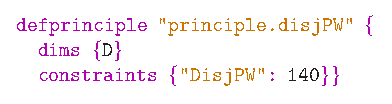
\includegraphics[scale=1.0]{eps/defprincipledisj}
\end{center}
% \begin{verbatim}
% functor
% export
%    Principle
% define
%    Principle =
%    elem(tag: principledef
% 	id: elem(tag: constant
% 		 data: 'principle.disjPW')
%         dimensions: [elem(tag: variable
%                           data: 'D')
%                     ]
%         constraints: [elem(tag: constant
%                            data: 'DisjPW')#
%                       elem(tag: integer
%                            data: 140)
%                      ])
% end
% \end{verbatim}
Und der Node-Constraint-Funktor sieht so aus:
\begin{center}
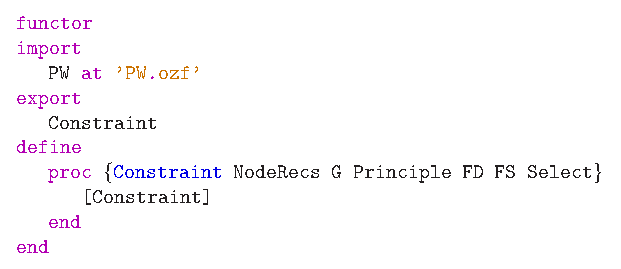
\includegraphics[scale=1.0]{eps/disjnc}
\end{center}
% \begin{verbatim}
% functor
% import
%    PW at 'PW.ozf'
% export
%    Constraint
% define
%    proc {Constraint NodeRecs G Principle FD FS Select}
%       [Constraint]
%    end
% end
% \end{verbatim}

\subsection{Die Funktionsbibliothek PW}

Die meisten Funktionen der {\tt PW}-Funktionsbibliothek geben die
Argumente direkt an die Funktionen der {\tt FD}- und {\tt
  FS}-Mozart/Oz Bibliotheken weiter, die Constraints \"uber endliche
Mengen und endliche Dom\"anen bereitstellen. Beispielhaft wollen wir
die Implementierung der Quantoren und der ungelabelten Kanten und
Pfade vorstellen.

\subsubsection{Die Quantoren der PW-Bibliothek}

Die Quantoren, die \"uber Knoten quantifizieren, deklarieren eine
unspezifizierte Mengenvariable $M$. Dann wird \"uber die Knoten,
\"uber die quantifiziert werden soll, iteriert. Bei jedem
Schleifendurchgang wird der aktuelle Knoten dann zur Menge $M$
hinzugef\"ugt, wenn die Formel im Rumpf des Quantors f\"ur den
aktuellen Knoten zu 1 auswertet.  Damit die $\forall$-Quantifizierung
wahr wird, muss nach der Iteration die Menge $M$ gleichm\"achtig der
Knotenmenge sein, \"uber die quantifiziert wurde.  Die
$\exists$-Quantifizierung wird wahr, wenn $M$ mindestens ein Element,
und die $\exists!$-Quantifizierug, wenn $M$ genau ein Element
enth\"alt. 

Die Quantoren \"uber die anderen Dom\"anen funktionieren \"ahnlich wie
die Knotenquantoren, mit dem Unterschied dass \"uber die Konstanten
der Dom\"ane, \"uber die quantifiziert wird, iteriert wird.

\subsubsection{Ungelabelte Kanten und Pfade der PW-Bibliothek}

Um zu pr\"ufen, ob es eine Kante von Knoten $v$ zu Knoten $v_1$ gibt,
wird getestet, ob $v_1$ in der Tochtermenge {\tt daughters} von $v$
ist. Ein Pfad von $v$ nach $v_1$ mit mindestens einer Kante existiert,
wenn $v_1$ in der {\tt down}-Menge von $v$ ist, ein Pfad mit
beliebiger Menge wird mit der {\tt eqdown} \"uberpr\"uft etc.
